\documentclass[11pt]{article}
\usepackage{geometry}                % See geometry.pdf to learn the layout options. There are lots.
\geometry{letterpaper}                   % ... or a4paper or a5paper or ... 
%\geometry{landscape}                % Activate for for rotated page geometry
\usepackage[parfill]{parskip}    % Activate to begin paragraphs with an empty line rather than an indent
\usepackage{daves,fancyhdr,natbib,graphicx,dcolumn,amsmath,lastpage,url}
\usepackage{amsmath,amssymb,epstopdf,longtable}
\usepackage{paralist}  % need to properly formulate standard answer blocks
\usepackage[final]{pdfpages}
\DeclareGraphicsRule{.tif}{png}{.png}{`convert #1 `dirname #1`/`basename #1 .tif`.png}
\pagestyle{fancy}
\lhead{CE 3372 Water Systems Design; Exam 2}
\rhead{Name:\_\_\_\_\_\_\_\_\_\_\_\_\_\_\_\_\_\_\_\_\_\_\_\_\_\_\_\_\_\_\_\_\_\_}
\lfoot{REVISION A \small{\#::}}
\cfoot{}
\rfoot{Page \thepage\ of \pageref{LastPage}}
\renewcommand\headrulewidth{0pt}
\newcommand\tab[1][1cm]{\hspace*{#1}}



\begin{document}
%%%%%%%%%%%%%%%%%%%%%%%%%%%%%%%%%%%
\begingroup
\begin{center}
{\textbf{{ CE 3372 Water Systems Design}  \\ Spring 2018} }
\end{center}
\endgroup

%%%%%%%%%%%%%%%%%%%%%%%%%%%
\begin{enumerate}
\item Consider the two networks depicted in Figure \ref{fig:TwoNetworks}.
Both network designs serve the same junction nodes, have same nodal demands, and draw supply from the same reservoir.
\begin{figure}[htbp] %  figure placement: here, top, bottom, or page
   \centering
   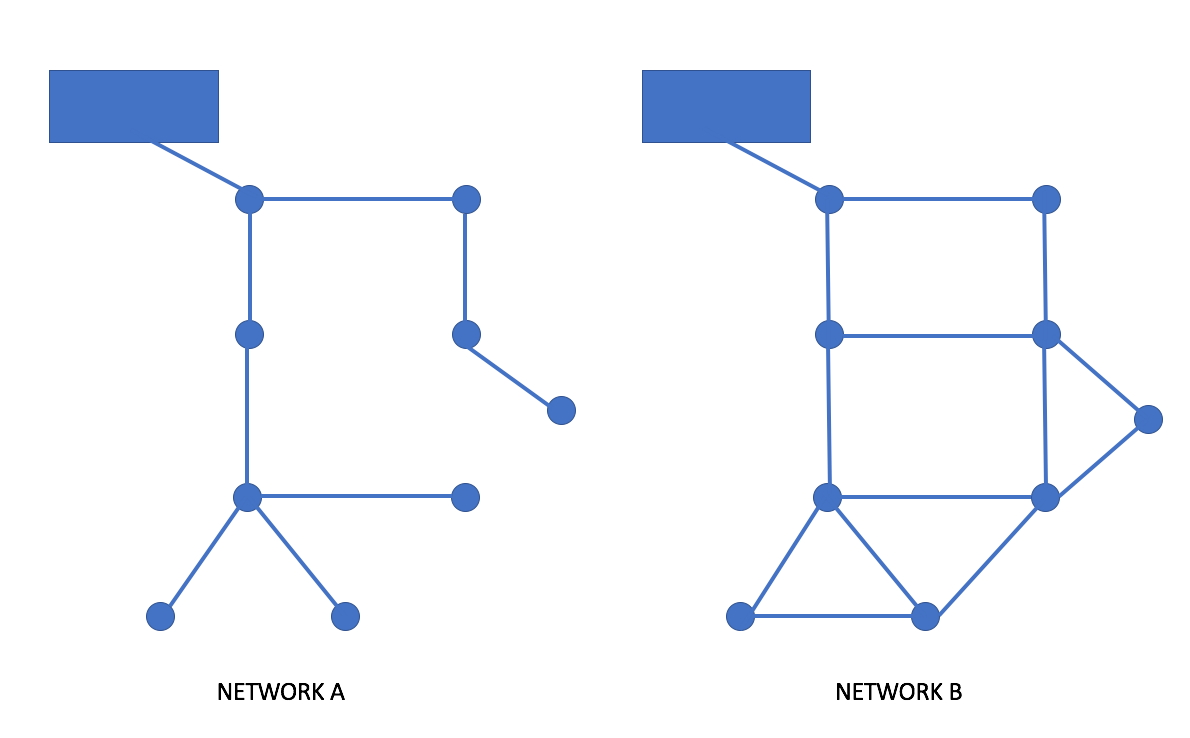
\includegraphics[width=5in]{TwoNetworks.jpg} 
   \caption{Two Network Designs}
   \label{fig:TwoNetworks}
\end{figure}
\begin{enumerate}[a)]
\item  Which network design would be superior in terms of reliability?   Why? \\~\\~\\~\\
\item Which network design would cost less to build?  Why? \\~\\~\\~\\
\item Which network would be superior in terms of disinfection residual? Why?
\end{enumerate}
\clearpage
\item Figure \ref{fig:EPANETWorkspace} is a screen capture of the EPANET graphical user interface.  Identify the following items in the workspace, and write the item names in the empty boxes on the figure.
\begin{enumerate}[a)]
\item Browser
\item Menu Bar
\item Network Map
\item Property Editor
\item Status Bar
\item Toolbars
\end{enumerate}
\begin{figure}[htbp] %  figure placement: here, top, bottom, or page
   \centering
   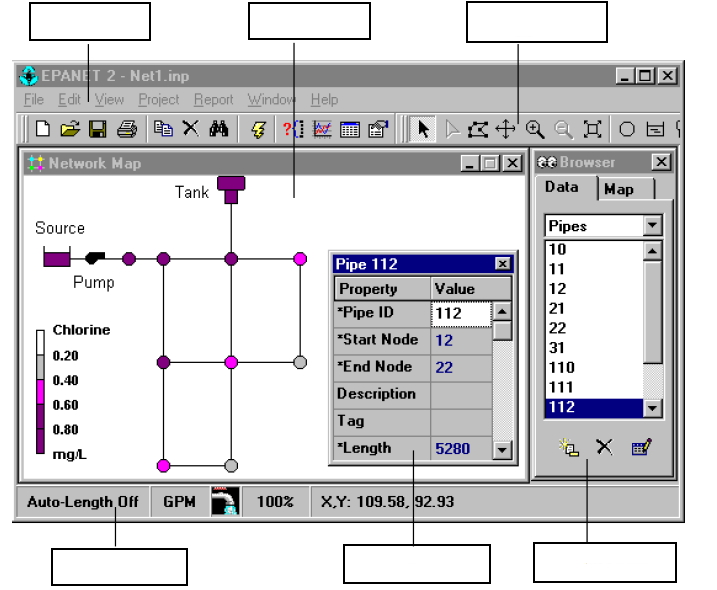
\includegraphics[width=6in]{EPANETWorkspace.jpg} 
   \caption{EPANET Workspace}
   \label{fig:EPANETWorkspace}
\end{figure}
\clearpage
\item Explain (using sketches as needed) how to model a groundwater pumping well in EPANET. \\~\\~\\~\\~\\~\\~\\~\\~\\~\\~\\~\\~\\~\\~\\~\\~\\~\\~\\
\item Explain (using sketches as needed) how to determine the maximum pressure available at a node when the demand at the node must be increased to suppress a fire. \\~\\~\\~\\~\\~\\~\\~\\~\\~\\
\item An EPANET model must have which of the following components to run
%standard answer set
\begin{enumerate}[a)]
\item A pipe, a node, and a pump 
\item A pipe, a node, and a valve
\item A pipe, a tank, and a pump
\item A pipe, a node, and a reservoir
\end{enumerate}



\clearpage
%%%%%%%%%%%%%%%%%%%%%%%%%%%%%%%%%%%%%%%%%%%%%%%
%%%%%%%% EPA PROBLEM BEGIN %%%%%%%%%%%%%%%%%%%%%%%%%%%
%%%%%%%%%%%%%%%%%%%%%%%%%%%%%%%%%%%%%%%%%%%%%%%
\item  An EPA-NET simulation model for a reservoir-pump-network was constructed and operated for four (4) different operational scenarios.   Figure \ref{fig:epa-net-map} is a depiction of the network.   The numbers next to the nodes are Node\_ID values in the reports that follow, and the numbers next to the pipes are the Link\_ID values.  The network is supplied from a reservoir through a booster pump, both are depicted on Figure \ref{fig:epa-net-map}. 

\begin{figure}[h!] %  figure placement: here, top, bottom, or page
\centering
   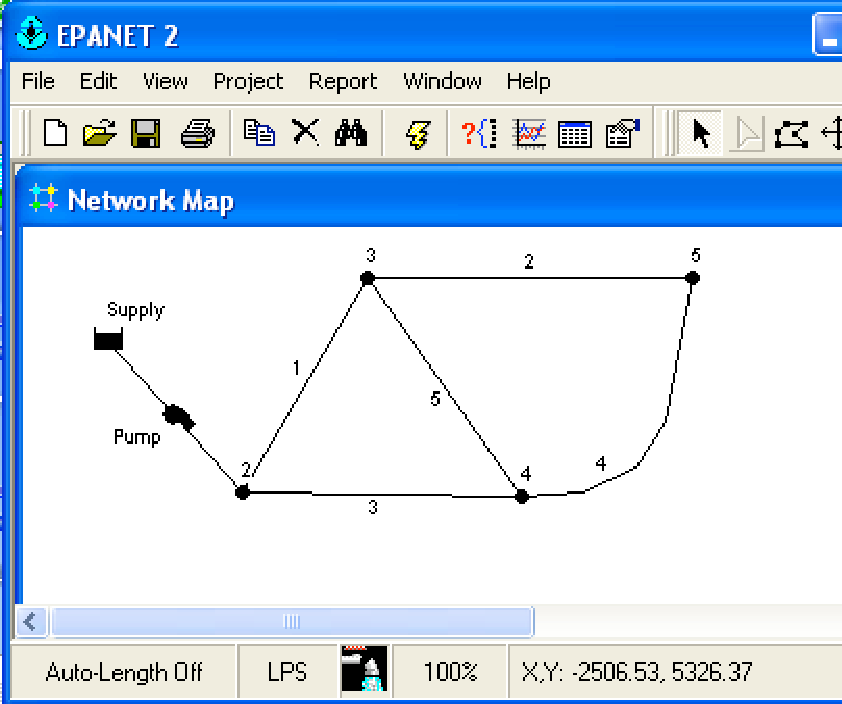
\includegraphics[width=3in]{epa-net-map.pdf}
   \caption{EPA-NET system topology.}
   \label{fig:epa-net-map} 
\end{figure}

Figure \ref{fig:epanet1} is the a portion of the summary report for simulation 1.   
Figure \ref{fig:epanet2} is the a portion of the summary report for simulation 2.  
Figure \ref{fig:epanet3} is the a portion of the summary report for simulation 3.  
Figure \ref{fig:epanet4} is the a portion of the summary report for simulation 4.

These four simulation represent different demand scenarios for the same system.



Interpret these reports, to answer the following questions:

\begin{enumerate}
\item Complete the table below.  $Q_{pump}$ is the discharge in liters-per-second through the pump station, $H_{Supply}$ is the head at the supply reservoir,  $H_{Node2}$ is the head at Node 2, and $\Delta H_{pump}$ is the added head supplied by the pump.
% Requires the booktabs if the memoir class is not being used
\begin{table}[htbp]
   \centering
      \caption{Pump Discharge and Supplied Head}
   \begin{tabular}{p{1in} p{1in} p{1in} p{1in} p{1in} } % Column formatting, @{} suppresses leading/trailing space
Simulation \# & $Q_{pump}$ & $H_{Supply}$ & $H_{Node2}$ & $\Delta H_{pump}$ \\
\hline
\hline
~~1 & ~ &~ & ~ & ~ \\
~ & ~ &~ & ~ & ~ \\
\hline
~~2 & ~ &~ & ~ & ~ \\
~ & ~ &~ & ~ & ~ \\
\hline
~~3 & ~ &~ & ~ & ~\\
~ & ~ &~ & ~ & ~ \\
\hline
~~4 & ~ &~ & ~ & ~ \\
~ & ~ &~ & ~ & ~ \\
\hline
   \end{tabular}
   \label{tab:pump-curve}
\end{table}

\item Complete the table below.  $Q_{pump}$ is the discharge in liters-per-second through the pump station, $\Delta H_{Node 2 -to- 5}$ is head loss in the system from Node 2 to Node 5.
\begin{table}[htbp]
   \centering
      \caption{System Discharge and Head Loss}
   \begin{tabular}{p{1in} p{1in} p{1in} p{1in} p{1in} } % Column formatting, @{} suppresses leading/trailing space
Simulation \# & $Q_{pump}$ & $H_{Node2}$ & $H_{Node5}$ & $\Delta H_{Node 2 -to- 5}$ \\
\hline
\hline
~~1 & ~ &~ & ~ & ~ \\
~ & ~ &~ & ~ & ~ \\
\hline
~~2 & ~ &~ & ~ & ~ \\
~ & ~ &~ & ~ & ~ \\
\hline
~~3 & ~ &~ & ~ & ~\\
~ & ~ &~ & ~ & ~ \\
\hline
~~4 & ~ &~ & ~ & ~ \\
~ & ~ &~ & ~ & ~ \\
\hline
   \end{tabular}
   \label{tab:system-curve}
\end{table}



\item If the pump performance curve has the mathematical structure: ~\\~\\
$\Delta H_{pump} = H_{shutoff} - C_{pump} \times Q^2$, estimate the values of $H_{shutoff}$  and $C_{pump}$.
\\
\\
\\
\\
\\
\\
\\
\\
\\
\\

\item If the system frictional loss curve has the mathematical structure:~\\~\\
 $H_{loss-system}= K_{network} \times Q^2$, estimate the value of $K_{network}$

\clearpage
\item What effect would removing the pipe joining nodes 3 and 4 have on the system performance?   Explain your reasoning.
\\
\\
\\
\\
\\
\\
\\
\\
\\
\\
\\
\\
\\
\item Estimate the flow distribution and head losses the the system if the the pipe joining nodes 3 and 4 are removed, and the pipe joining node 4 and 5 is removed if the nodal demands are the same as SIMULATION  2.
\end{enumerate} 

%%% YOUR ON YOUR OWN %%%%%%%%%%%%%%%%%%%%
\begin{figure}[ht!] %  figure placement: here, top, bottom, or page
\centering

\begin{verbatim}
  Page 1                                            10/4/2010 2:27:47 PM
  **********************************************************************
  *                             E P A N E T                            *
  *                     Hydraulic and Water Quality                    *
  *                     Analysis for Pipe Networks                     *
  *                           Version 2.0                              *
  **********************************************************************
  Input File: SIMULATION #1
Link - Node Table:
  ----------------------------------------------------------------------
  Link           Start          End                Length  Diameter
  ID             Node           Node                    m        mm
  ----------------------------------------------------------------------
  1              2              3                    1000       124
  2              3              5                    1000       124
  3              2              4                    1000       124
  4              4              5                    1000       124
  5              3              4                    1400       124
  7              6              2                    #N/A      #N/A Pump
Node Results:
  ----------------------------------------------------------------------
  Node                Demand      Head  Pressure   Quality
  ID                     LPS         m         m          
  ----------------------------------------------------------------------
  2                     0.00     20.00     20.00      0.00
  3                     0.00     20.00     20.00      0.00
  4                     0.00     20.00     20.00      0.00
  5                     0.00     20.00     20.00      0.00
  6                     0.00      0.00      0.00      0.00 Reservoir
Link Results:
  ----------------------------------------------------------------------
  Link                  Flow  VelocityUnit Headloss    Status
  ID                     LPS       m/s      m/km
  ----------------------------------------------------------------------
  1                     0.00      0.00      0.00      Open
  2                     0.00      0.00      0.00      Open
  3                     0.00      0.00      0.00      Open
  4                     0.00      0.00      0.00      Open
  5                     0.00      0.00      0.00      Open
  7                     0.00      0.00    -20.00      Open Pump
  \end{verbatim}
     \caption{EPA-NET Summary Report, Simulation \#1}
   \label{fig:epanet1} 
\end{figure}


\begin{figure}[ht!] %  figure placement: here, top, bottom, or page
\centering
\begin{verbatim}
 Page 1                                            10/4/2010 2:28:15 PM
  **********************************************************************
  *                             E P A N E T                            *
  *                     Hydraulic and Water Quality                    *
  *                     Analysis for Pipe Networks                     *
  *                           Version 2.0                              *
  **********************************************************************
  Input File: SIMULATION 2
  Link - Node Table:
  ----------------------------------------------------------------------
  Link           Start          End                Length  Diameter
  ID             Node           Node                    m        mm
  ----------------------------------------------------------------------
  1              2              3                    1000       124
  2              3              5                    1000       124
  3              2              4                    1000       124
  4              4              5                    1000       124
  5              3              4                    1400       124
  7              6              2                    #N/A      #N/A Pump
  Node Results:
  ----------------------------------------------------------------------
  Node                Demand      Head  Pressure   Quality
  ID                     LPS         m         m          
  ----------------------------------------------------------------------
  2                     0.00     19.28     19.28      0.00
  3                     1.00     19.03     19.03      0.00
  4                     1.00     19.03     19.03      0.00
  5                     1.00     18.99     18.99      0.00
  6                    -3.00      0.00      0.00      0.00 Reservoir                                                              
  Link Results:
  ----------------------------------------------------------------------
  Link                  Flow  VelocityUnit Headloss    Status
  ID                     LPS       m/s      m/km
  ----------------------------------------------------------------------
  1                     1.50      0.12      0.25      Open
  2                     0.50      0.04      0.03      Open
  3                     1.50      0.12      0.25      Open
  4                     0.50      0.04      0.03      Open
  5                     0.00      0.00      0.00      Open
  7                     3.00      0.00    -19.28      Open Pump
  \end{verbatim}
     \caption{EPA-NET Summary Report, Simulation \#2}
   \label{fig:epanet2} 
\end{figure}

\begin{figure}[ht!] %  figure placement: here, top, bottom, or page
\centering

\begin{verbatim}
   Page 1                                            10/4/2010 2:29:00 PM
  **********************************************************************
  *                             E P A N E T                            *
  *                     Hydraulic and Water Quality                    *
  *                     Analysis for Pipe Networks                     *
  *                           Version 2.0                              *
  **********************************************************************
  Input File: SIMULATION 3
 Link - Node Table:
  ----------------------------------------------------------------------
  Link           Start          End                Length  Diameter
  ID             Node           Node                    m        mm
  ----------------------------------------------------------------------
  1              2              3                    1000       124
  2              3              5                    1000       124
  3              2              4                    1000       124
  4              4              5                    1000       124
  5              3              4                    1400       124
  7              6              2                    #N/A      #N/A Pump
Node Results:
  ----------------------------------------------------------------------
  Node                Demand      Head  Pressure   Quality
  ID                     LPS         m         m          
  ----------------------------------------------------------------------
  2                     0.00     17.12     17.12      0.00
  3                     2.00     16.16     16.16      0.00
  4                     2.00     16.16     16.16      0.00
  5                     2.00     16.04     16.04      0.00
  6                    -6.00      0.00      0.00      0.00 Reservoir
Link Results:
  ----------------------------------------------------------------------
  Link                  Flow  VelocityUnit Headloss    Status
  ID                     LPS       m/s      m/km
  ----------------------------------------------------------------------
  1                     3.00      0.25      0.96      Open
  2                     1.00      0.08      0.12      Open
  3                     3.00      0.25      0.96      Open
  4                     1.00      0.08      0.12      Open
  5                     0.00      0.00      0.00      Open
  7                     6.00      0.00    -17.12      Open Pump
  \end{verbatim}
     \caption{EPA-NET Summary Report, Simulation \#3}
   \label{fig:epanet3} 
\end{figure}

\begin{figure}[ht!] %  figure placement: here, top, bottom, or page
\centering

\begin{verbatim}
  Page 1                                            10/4/2010 2:29:46 PM
  **********************************************************************
  *                             E P A N E T                            *
  *                     Hydraulic and Water Quality                    *
  *                     Analysis for Pipe Networks                     *
  *                           Version 2.0                              *
  **********************************************************************
  Input File: SIMULATION 4
Link - Node Table:
  ----------------------------------------------------------------------
  Link           Start          End                Length  Diameter
  ID             Node           Node                    m        mm
  ----------------------------------------------------------------------
  1              2              3                    1000       124
  2              3              5                    1000       124
  3              2              4                    1000       124
  4              4              5                    1000       124
  5              3              4                    1400       124
  7              6              2                    #N/A      #N/A Pump
Node Results:
  ----------------------------------------------------------------------
  Node                Demand      Head  Pressure   Quality
  ID                     LPS         m         m          
  ----------------------------------------------------------------------
  2                     0.00     13.52     13.52      0.00
  3                     3.00     11.40     11.40      0.00
  4                     3.00     11.40     11.40      0.00
  5                     3.00     11.15     11.15      0.00
  6                    -9.00      0.00      0.00      0.00 Reservoir
 Link Results:
  ----------------------------------------------------------------------
  Link                  Flow  VelocityUnit Headloss    Status
  ID                     LPS       m/s      m/km
  ----------------------------------------------------------------------
  1                     4.50      0.37      2.12      Open
  2                     1.50      0.12      0.25      Open
  3                     4.50      0.37      2.12      Open
  4                     1.50      0.12      0.25      Open
  5                     0.00      0.00      0.00      Open
  7                     9.00      0.00    -13.52      Open Pump
  \end{verbatim}
     \caption{EPA-NET Summary Report, Simulation \#4}
   \label{fig:epanet4} 
\end{figure}
\clearpage

%%%%%%%%%%%%%%%%%%%%%%%%%%%%%%%%%%%%%%%%%%%%%%
%%%%%%%% PROBLEM 1 %%%%%%%%%%%%%%%%%%%%%%%%%%%%%%%
%%%%%%%%%%%%%%%%%%%%%%%%%%%%%%%%%%%%%%%%%%%%%%
\item  The hydraulic radius in a conduit containing a flowing liquid is
\begin{enumerate} [(A)]
\item	the mean radius from the center of flow to the wetted side of the conduit
\item	the ratio of the cross-sectional area of the conduit and the wetted perimeter
\item	the ratio of the wetted perimeter and the cross-sectional area of the conduit
\item	the ratio of the cross-sectional area of flow and the wetted perimeter
\end{enumerate}
%\item  A pipe with a diameter of $2.4$ meters is depicted in Figure \ref{fig:CircularSewerToo}.   The pipe is flowing partially full.
%
%\begin{figure}[h!] %  figure placement: here, top, bottom, or page
%\centering
%   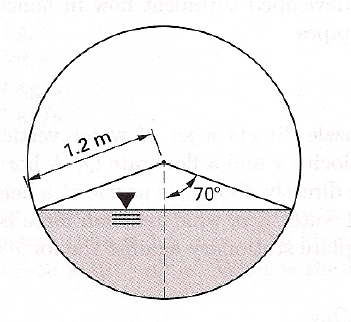
\includegraphics[width=1.9in]{CircularSewerToo.jpg}
%   \caption{Circular channel flowing partially full.}
%   \label{fig:CircularSewerToo} 
%\end{figure}
%
%
%~\clearpage

\item A circular, 60-inch diameter, reinforced concrete sewer pipe ($n = 0.013$ )carries 50 MGD of wastewater to a lift station wet well.   Average slope along the flow path is 1.0\%.

\begin{enumerate} [a)]
\item	Sketch the cross section, indicate the pipe diameter.
~\\
~\\
~\\
~\\
~\\
~\\
~\\
~\\
~\\
~\\
~\\
~\\
\item For the conditions in the problem statement, what is the flow rate in cubic feet per second?
~\\

\item What is the diameter of the pipe, in feet?
~\\

\item Use Manning's equation ($ Q = \frac{1.49}{n} A R^{(2/3)} S^{(1/2)} $) and determine the \textbf{pipe-full} discharge in cubic feet per second. ~\\~\\~\\~\\~\\~\\~\\~\\~\\
\item What is the pipe-full discharge ($Q_{f}$) in million gallons per day (MGD)? ~\\~\\~\\~\\~\\
%
\item Determine the discharge in the sewer when it is half-full, in million gallons per day (MGD). ~\\~\\~\\~\\~\\~\\~\\~\\~\\~\\
\item Determine the discharge in the sewer when it is 90\%full, in million gallons per day (MGD). ~\\~\\~\\~\\~\\~\\~\\~\\~\\~\\
\item Determine the discharge in the sewer when it is 75\%full, in million gallons per day (MGD). ~\\~\\~\\~\\~\\~\\~\\~\\~\\~\\
\item Which of these conditions (50\%,75\%,90\% of full) is closest to the actual flow of 50 MGD? 
\end{enumerate}
\clearpage

14. A smooth concrete channel is depicted in Figure \ref{fig:TriangleChannel}.  The channel's dimensionless slope in the direction of flow is $0.005$.  If the flow width at the surface is $2$-meter, what is the flow rate in the channel?

\begin{figure}[h!] %  figure placement: here, top, bottom, or page
\centering
   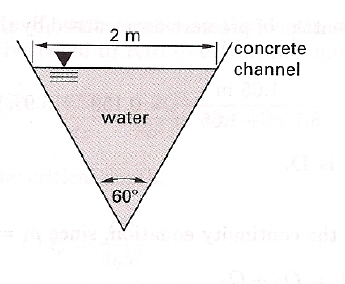
\includegraphics[width=2.2in]{TriangleChannel.jpg}
   \caption{Triangular channel.}
   \label{fig:TriangleChannel} 
\end{figure}
\clearpage


%%%%%%%%%%%%%%%%%%%%%%%%%%%%%%%%%%%%%%%%%%%%%%
%%%%%%%% PROBLEM 2 %%%%%%%%%%%%%%%%%%%%%%%%%%%%%%%
%%%%%%%%%%%%%%%%%%%%%%%%%%%%%%%%%%%%%%%%%%%%%%
\item The rational runoff coefficient for a $14.81$~acre parcel property is $0.35$.  
The rainfall intensity is $4.56$ inches per hour.    
Determine the size (diameter) of a reinforced concrete sewer pipe to convey the peak discharge, if the pipe is to be laid on a 0.5\% slope, and the desired flow depth in the pipe is 1/2 full.
%\clearpage
%\item List the names of your water systems team members in the table below.  Rate them in the categories indicated, from 1 to 4 with 1 being poor performance, and 4 bring excellent performance.
%\begin{table}[htbp]
%   \centering
%      \caption{Mid-term Team Mate Assessment}
%   \begin{tabular}{p{2in} p{0.9in} p{0.9in} p{0.9in} p{0.7in} } % Column formatting, @{} suppresses leading/trailing space
% ~ & ~ & ~ & ~ & ~ \\
% \hline
% \hline
%Team Member Name & Reliability & Availability & Work Quality & Contribution(\%) \\
%\hline
% 1)~ & ~ & ~ & ~ & ~ \\
%  ~ & ~ & ~ & ~ & ~ \\
%    ~ & ~ & ~ & ~ & ~ \\
%      ~ & ~ & ~ & ~ & ~ \\
%  \hline
% 2) ~ & ~ & ~ & ~ & ~ \\
%  ~ & ~ & ~ & ~ & ~ \\
%    ~ & ~ & ~ & ~ & ~ \\
%      ~ & ~ & ~ & ~ & ~ \\
%  \hline
%3)  ~ & ~ & ~ & ~ & ~ \\
%  ~ & ~ & ~ & ~ & ~ \\
%    ~ & ~ & ~ & ~ & ~ \\
%      ~ & ~ & ~ & ~ & ~ \\
%  \hline
%4)   ~ & ~ & ~ & ~ & ~ \\
%  ~ & ~ & ~ & ~ & ~ \\
%    ~ & ~ & ~ & ~ & ~ \\
%      ~ & ~ & ~ & ~ & ~ \\
%  \hline
%5)  ~ & ~ & ~ & ~ & ~ \\
%  ~ & ~ & ~ & ~ & ~ \\
%    ~ & ~ & ~ & ~ & ~ \\
%      ~ & ~ & ~ & ~ & ~ \\
%  \hline
%   \end{tabular}
%   \label{tab:system-curve}
%\end{table}
%~\\Additional Comments Below: \footnote{This sheet will be removed from the exam and will not be returned, the feedback is used to assess team effectiveness, but does not affect the examination score.}
%\item The rational runoff coefficient for a $300X200$-meter property with a slope of $3$\% is $0.35$.  The rainfall intensity is $116$ mm/hr.  The peak discharge from this property is anticipated to be about
%%standard answer set
%\begin{enumerate} [(A)]
%\item $2200~m^3/hr$
%\item $2400~m^3/hr$
%\item $3800~m^3/hr$
%\item $7000~m^3/hr$
%\end{enumerate}
%======== SOLUTION ===========
% B   Apply Rational Runoff Formula (in SI units)
% NCEES pp 159
%=============================
%
%%%%%%%%%%%%%%%%%%%%%%%%%%%%%%%%%%%%%%%%%%%%%%
%%%%%%%% PROBLEM 6 BEGIN %%%%%%%%%%%%%%%%%%%%%%%%%%%
%%%%%%%%%%%%%%%%%%%%%%%%%%%%%%%%%%%%%%%%%%%%%%
%%%%%%%%%%%%%%%%%%%%%%%%%%%%%%%%%%%%%%%%%%%%%%
%%%%%%%% PROBLEM 2 DONE %%%%%%%%%%%%%%%%%%%%%%%%%%%
%%%%%%%%%%%%%%%%%%%%%%%%%%%%%%%%%%%%%%%%%%%%%%






\end{enumerate}

\end{document}  




